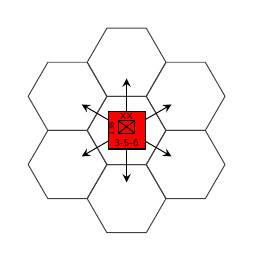
\begin{tikzpicture}[
  x=1cm,
  y=1cm,
  line cap=round,
  line join=round,
  zoc hex/.style={draw=black!75, line width=0.35pt},
  zoc arrow/.style={->, >=stealth, line width=0.35pt}
]
  \def\hexradius{0.50}

  % The occupied hex and the six surrounding hexes in its ZOC.
  \foreach \x/\y in {
    0/0,
    0/0.866,
    0/-0.866,
    0.75/0.433,
    0.75/-0.433,
    -0.75/0.433,
    -0.75/-0.433
  } {
    \draw[zoc hex, shift={(\x,\y)}]
      (0:\hexradius) -- (60:\hexradius) -- (120:\hexradius) --
      (180:\hexradius) -- (240:\hexradius) -- (300:\hexradius) -- cycle;
  }

  % Arrows show the unit projecting its ZOC into every adjacent hex.
  \draw[zoc arrow] (0,0.22) -- (0,0.66);
  \draw[zoc arrow] (0,-0.22) -- (0,-0.66);
  \draw[zoc arrow] (0.19,0.11) -- (0.57,0.33);
  \draw[zoc arrow] (0.19,-0.11) -- (0.57,-0.33);
  \draw[zoc arrow] (-0.19,0.11) -- (-0.57,0.33);
  \draw[zoc arrow] (-0.19,-0.11) -- (-0.57,-0.33);

  % Soviet 138th Rifle Division counter.
  \filldraw[fill=red, draw=black, line width=0.4pt]
    (-0.235,-0.235) rectangle (0.235,0.235);
  \node[font=\sffamily\tiny, scale=0.65] at (0,0.185) {XX};
  \node[rotate=90, font=\sffamily\tiny, scale=0.58]
    at (-0.195,0.02) {138};
  \draw[line width=0.35pt] (-0.105,0.125) rectangle (0.105,-0.035);
  \draw[line width=0.35pt] (-0.105,0.125) -- (0.105,-0.035);
  \draw[line width=0.35pt] (-0.105,-0.035) -- (0.105,0.125);
  \node[font=\sffamily\tiny, scale=0.75] at (0,-0.155) {3-5-6};
\end{tikzpicture}
